\chapter{Szabályozó modellezése}\label{chap:controller}

Az~\ref{chap:observer}.\ fejezetben levezetett állapotmegfigyelő és a szögelfordulás közvetlen mérése
együtt a rendszer teljes állapotvektorát elérhetővé teszi. Az impedancia modell által előírt dinamikai összefüggés
első lépésben teljes állapotvisszacsatolással biztosítható. A rendszer pólusai a~\ref{chap:controllability}.\ fejezetben
vizsgált irányíthatósági feltétel teljesülése miatt szabadon áthelyezhetők.

\section{Pozíció szabályozás}
Az előírt modell két független bemenettel rendelkezik. Jelen esetben a szögelfordulásra és a 
külső nyomatékra adott válasz viszont csak az amplitúdójukban térnek el. Ezt kihasználva először kizárólag a szögelfordulás referencia jelére előírt válasz alapján 
kerülnek áthelyezésre a pólusok. Teljes állapotvisszacsatolás esetén a motorra kapcsolt feszültség
\begin{align}\label{eq:position_control_voltage}
    V = K_\RM r \theta_\RM r -\BF K \tilde{\BF x}
\end{align}
összefüggéssel adható meg, 
ahol $\BF K$ az állapotvisszacsatolási mátrix, 
$K_\RM r$ a referencia jel erősítési tényezője és
$\theta_\RM r$ az előírt szögelfordulás. A~\eqref{eq:position_control_voltage} egyenletet felhasználásával
a~\eqref{eq:state_space_generic} egyenletben szereplő állapottér modell belső állapotának dinamikája
\begin{align}\label{eq:position_control_law_state}
    \dot{\BF x} = \BF A \BF x + \BF B_\RM V\left[K_\RM r \theta_\RM r - \BF K \tilde{\BF x}\right] + \BF B_\RM \tau \tau_\RM e,
\end{align}
alakra írható át. A $\BF B$ mátrix oszlopai elkülönítve $\BF B_\RM V$ és $\BF B_\RM \tau$ paraméterekként jelennek meg.
Legyen a továbbiakban a motor becsült állapotai és a megfigyelő által számított állapotok közötti hiba:
\begin{align}
    \BF e = \BF x_\RM b - \tilde{\BF x}_\RM b\,.
\end{align}
A~\eqref{eq:position_control_law_state} egyenlet a megfigyelő által számított állapotok 
vektorának kiküszöbölésével
\begin{align}
    \dot{\BF x} = \left(\BF A - \BF B_\RM V \BF K\right) \BF x + 
    \BF B_\RM V \BF K_\RM b \BF e + 
    \BF B_\RM \tau \tau + 
    \BF B_\RM V K_\RM r \theta_\RM r,
\end{align}
alakra hozható. A valós és becsült állapot közötti hiba dinamikája~\eqref{eq:observer_state} felhasználásával
\begin{equation}
    \begin{split}
    \dot{\BF x}_\RM b &= \BF A_\RM{ba} x_\RM a + \BF A_\RM{bb} \BF x_\RM b + 
    \BF B_\RM{Vb} V + \BF B_\RM{\tau b} \tau_\RM e\,,\\
    \dot{\tilde{\BF x}}_\RM b &= \left(\BF A_\RM{bb} - \BF K_\RM e \BF A_\RM{ab}\right) \tilde{\BF x}_\RM b +
    \BF A_\RM{ba} x_\RM a +
    \BF K_\RM e \BF A_\RM{ab} \BF x_\RM b +
    \BF B_\RM{Vb} V\,,
    \end{split}
\end{equation}
melyeket kivonva egymásból
\begin{align}
    \dot{\BF e} = \left(\BF A_\RM{bb} - \BF K_\RM e \BF A_\RM{ab}\right) \BF e + \BF B_\RM{\tau b} \tau_\RM e\,.
\end{align}
A rendszer dinamikája blokk mátrix alakban
\begin{align}\label{eq:pos_control_dynamics}
    \begin{bmatrix}
        \dot{\BF x} \\
        \dot{\BF e}
    \end{bmatrix}
    =
    \begin{bmatrix}
        \BF A - \BF B_\RM V \BF K & \BF B_\RM V \BF K_\RM b \\
        \BF 0 & \BF A_\RM{bb} - \BF K_\RM e \BF A_\RM{ab}
    \end{bmatrix}
    \begin{bmatrix}
        \BF x \\
        \BF e
    \end{bmatrix}
    +
    \begin{bmatrix}
        \BF B_\RM \tau & \BF B_\RM V K_\RM r\\
        \BF B_\RM{\tau b} & \BF 0
    \end{bmatrix}
    \begin{bmatrix}
        \tau_\RM e \\
        \theta_\RM r
    \end{bmatrix}.
\end{align}

A referencia jel erősítési tényezője a teljes rendszer átviteli függvénye alapján a végérték tétellel határozható meg.
A rendszer válaszának végértéke~\eqref{eq:pos_control_dynamics} szerint egységugrás bemenetre:
\begin{equation}
    \lim_{s \to 0}~s \cdot \theta(s) = 
    \lim_{s \to 0}~-\frac{K_\RM m K_\RM r M_\RM e}{JL(p-s)(M_\RM e s^2 + B_\RM e s + K_\RM e)}\frac{s}{s} =
    -\frac{K_\RM m K_\RM r M_\RM e}{JLpK_\RM e}\,,
\end{equation}
ahol \(p\) a függetlenül választható pólus. Az erősítési tényező ez alapján:
\begin{equation}\label{eq:input_coeff}
    K_\RM r = -\frac{JLpK_\RM e}{K_\RM m M_\RM e}\,.
\end{equation}

A megfigyelő belső hibájának (\(\BF e\)) megváltozása nem csak a pillanatnyi belső hibától függ. Még ha \(\BF A_\RM{bb} - \BF K_\RM e \BF A_\RM{ab}\) sajátértékei
mind negatív valós résszel is rendelkeznek, a megfigyelő belső hibája akkor sem tart nullához külső nyomaték jelenlétében.
Amennyiben \(\BF A - \BF B_\RM V \BF K\) sajátértékei is mind negatív valós résszel rendelkeznek,
a teljes rendszer exponenciálisan stabil, de a külső nyomatékra adott válasz végértéke eltér az impedancia modell
által előírt értéktől. Ez a szabályozó még nem felel meg az alkalmazás előírásainak. A rendszer válasza a pozíció referencia bemenetre adott egységugrás jelre a~\ref{fig:observer_controller_pos_resp}. ábrán látható. 
Az alkalmazott paramétereket az~\ref{tab:observer_controller_pos_resp}. táblázat tartalmazza. 
\begin{figure}[ht]
    \begin{center}
    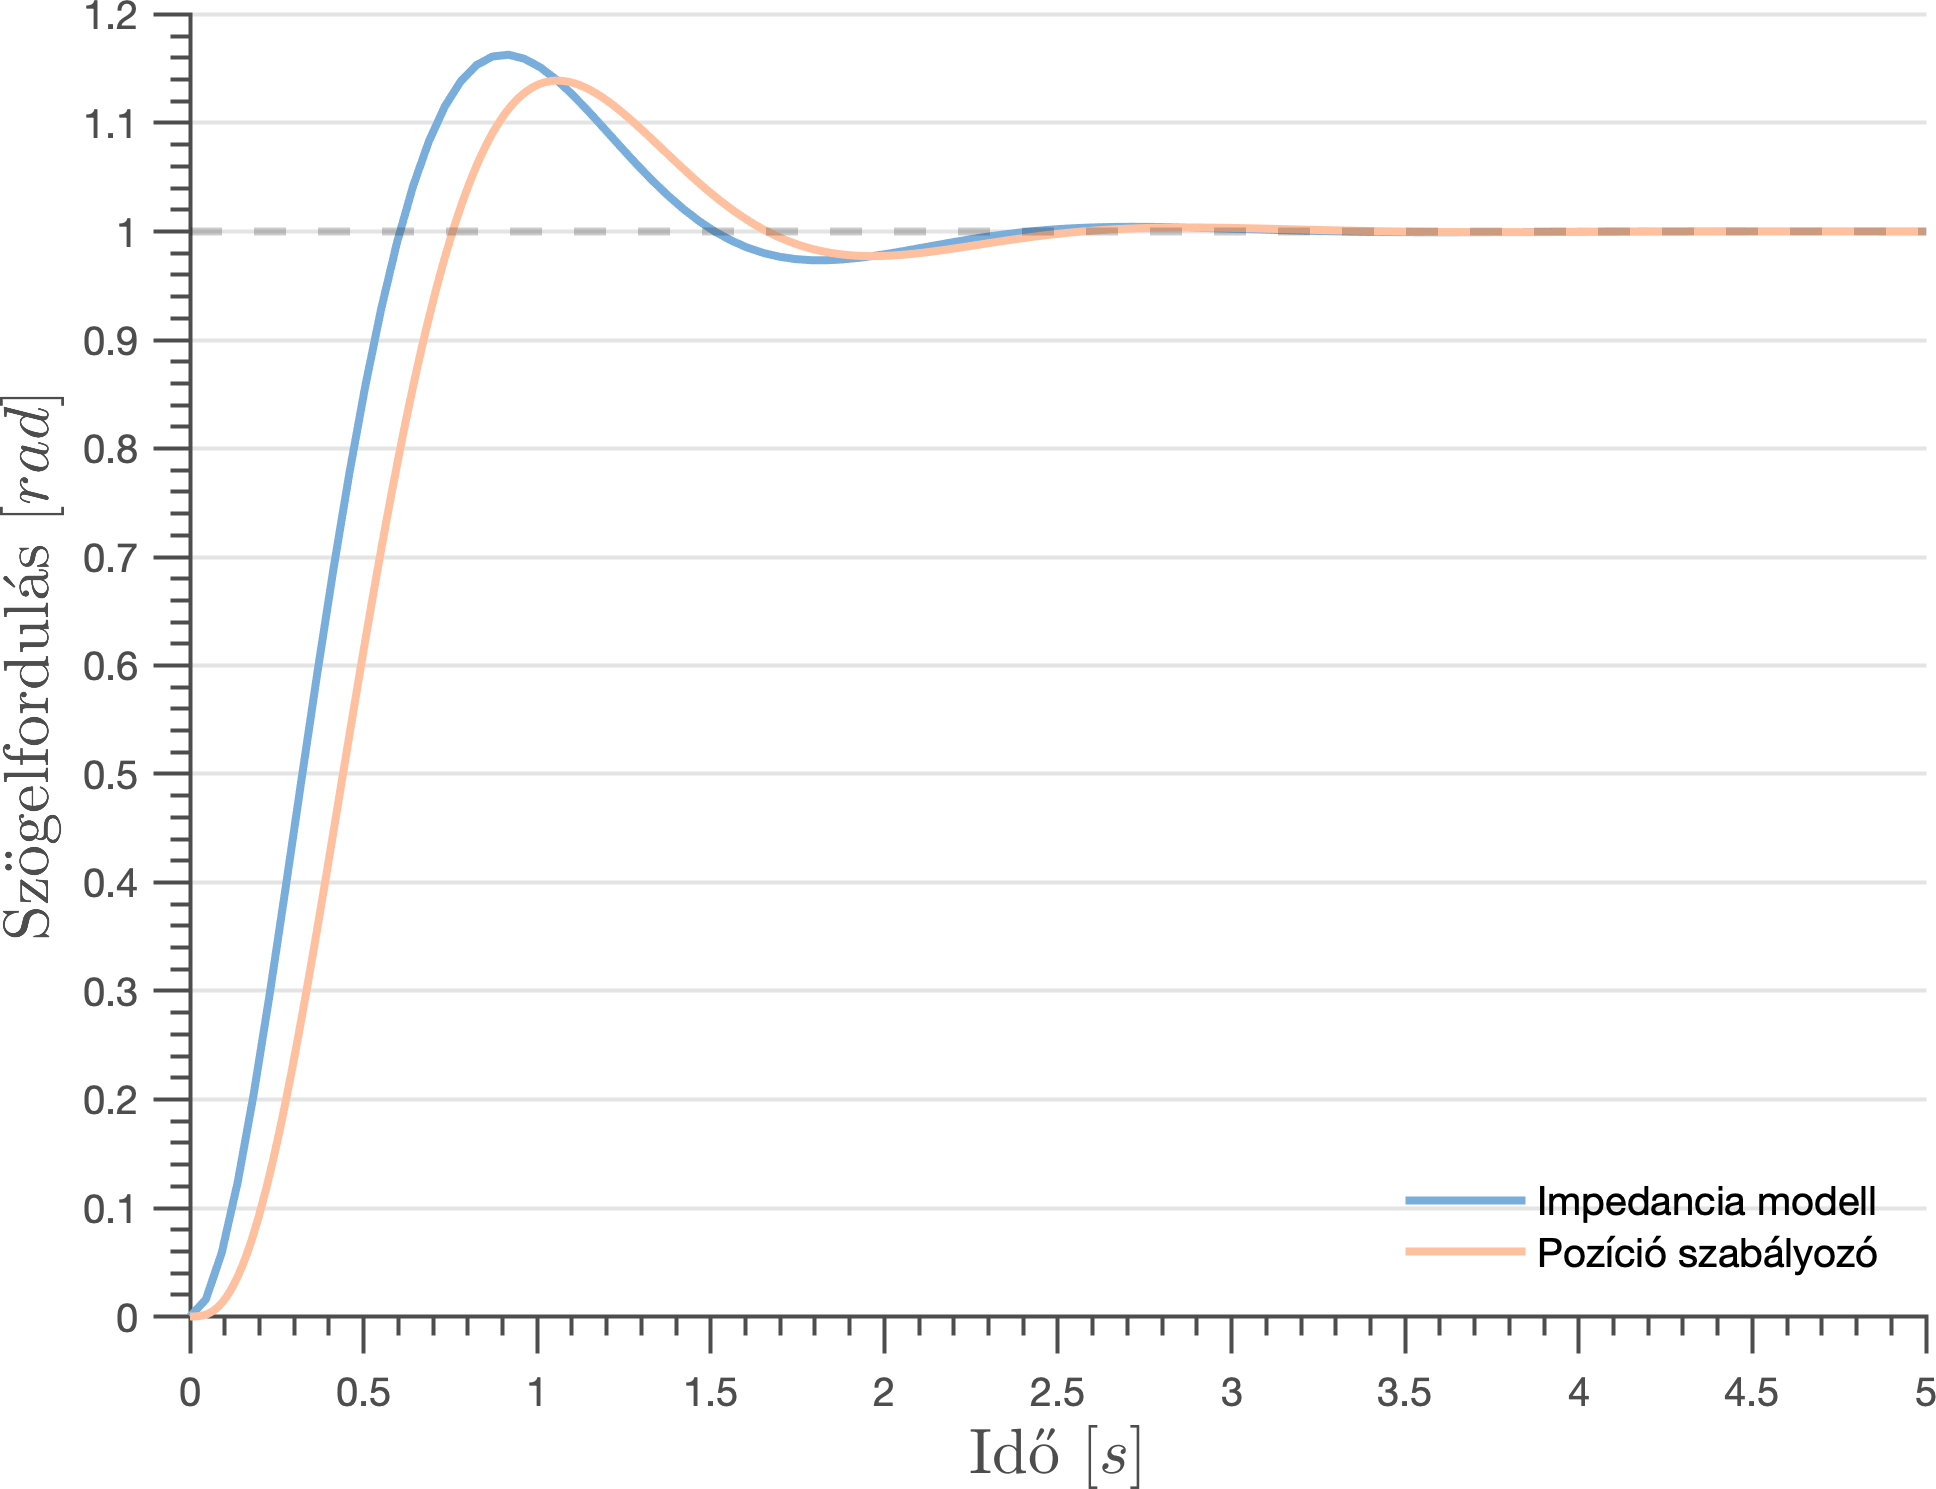
\includegraphics[width=\textwidth]{images/observer_controller_pos_resp.png}
    \caption{Az impedancia modell és a szabályozó összehasonlítása pozíció egységugrás bemenetre}\label{fig:observer_controller_pos_resp}
    \end{center}
\end{figure}

\begin{table}[ht]
    \small\centering
    \caption{Pozíció referencia bemenetre adott egységugrás jelnél alkalmazott paraméterek}\label{tab:observer_controller_pos_resp}
    \tabcolsep=1pt
    \begin{tabular}{l>{~}l>{\quad}rl}
        \toprule
        \multicolumn{2}{c}{Szimbólum és paraméter név} & \multicolumn{2}{c}{Érték} \\ \midrule
        \(M_\RM e\) & Előírt tehetetlenség & 1 & \(\RM{kg\cdot m^2}\) \\
        \(B_\RM e\) & Előírt viszkózus csillapítás & 4 & \(\RM{kg\cdot m^2\cdot s^{-1}}\) \\
        \(K_\RM e\) & Előírt rugóállandó & 16 & \(\RM{kg\cdot m^2\cdot s^{-2}}\) \\
        \(J\) & Motor tehetetlensége & 0.01 & \(\RM{kg\cdot m^2}\) \\
        \(K_\RM m\) & Motor nyomatékállandója & 0.01 & \(\RM{Nm\cdot A^{-1}}\) \\
        \(B_\RM m\) & Motor modell viszkózus csillapítása & 0.1 & \(\RM{kg\cdot m^2\cdot s^{-1}}\) \\
        \(L\) & Motor induktivitása & 0.2 & H \\
        \(R\) & Motor ellenállása & 1 & \(\Omega\) \\
        \bottomrule
    \end{tabular}
\end{table}

Az áthelyezett pólusok \(P = [-2.00 - 3.46i~~-2.00 + 3.46i~~-8.00]\) 
és a megfigyelő pólusai \(P_\RM o = [-8.00~~-8.00]\). Az első két áthelyezett pólust az impedancia modell
határozza meg. A többi pólus meghatározásához szükséges feltételek vizsgálata a nyomatékválasz vizsgálata után következik.
A pólusok alapján a visszacsatolási mátrixok az Ackermann formulával lettek meghatározva.

\begin{figure}[ht]
    \begin{center}
    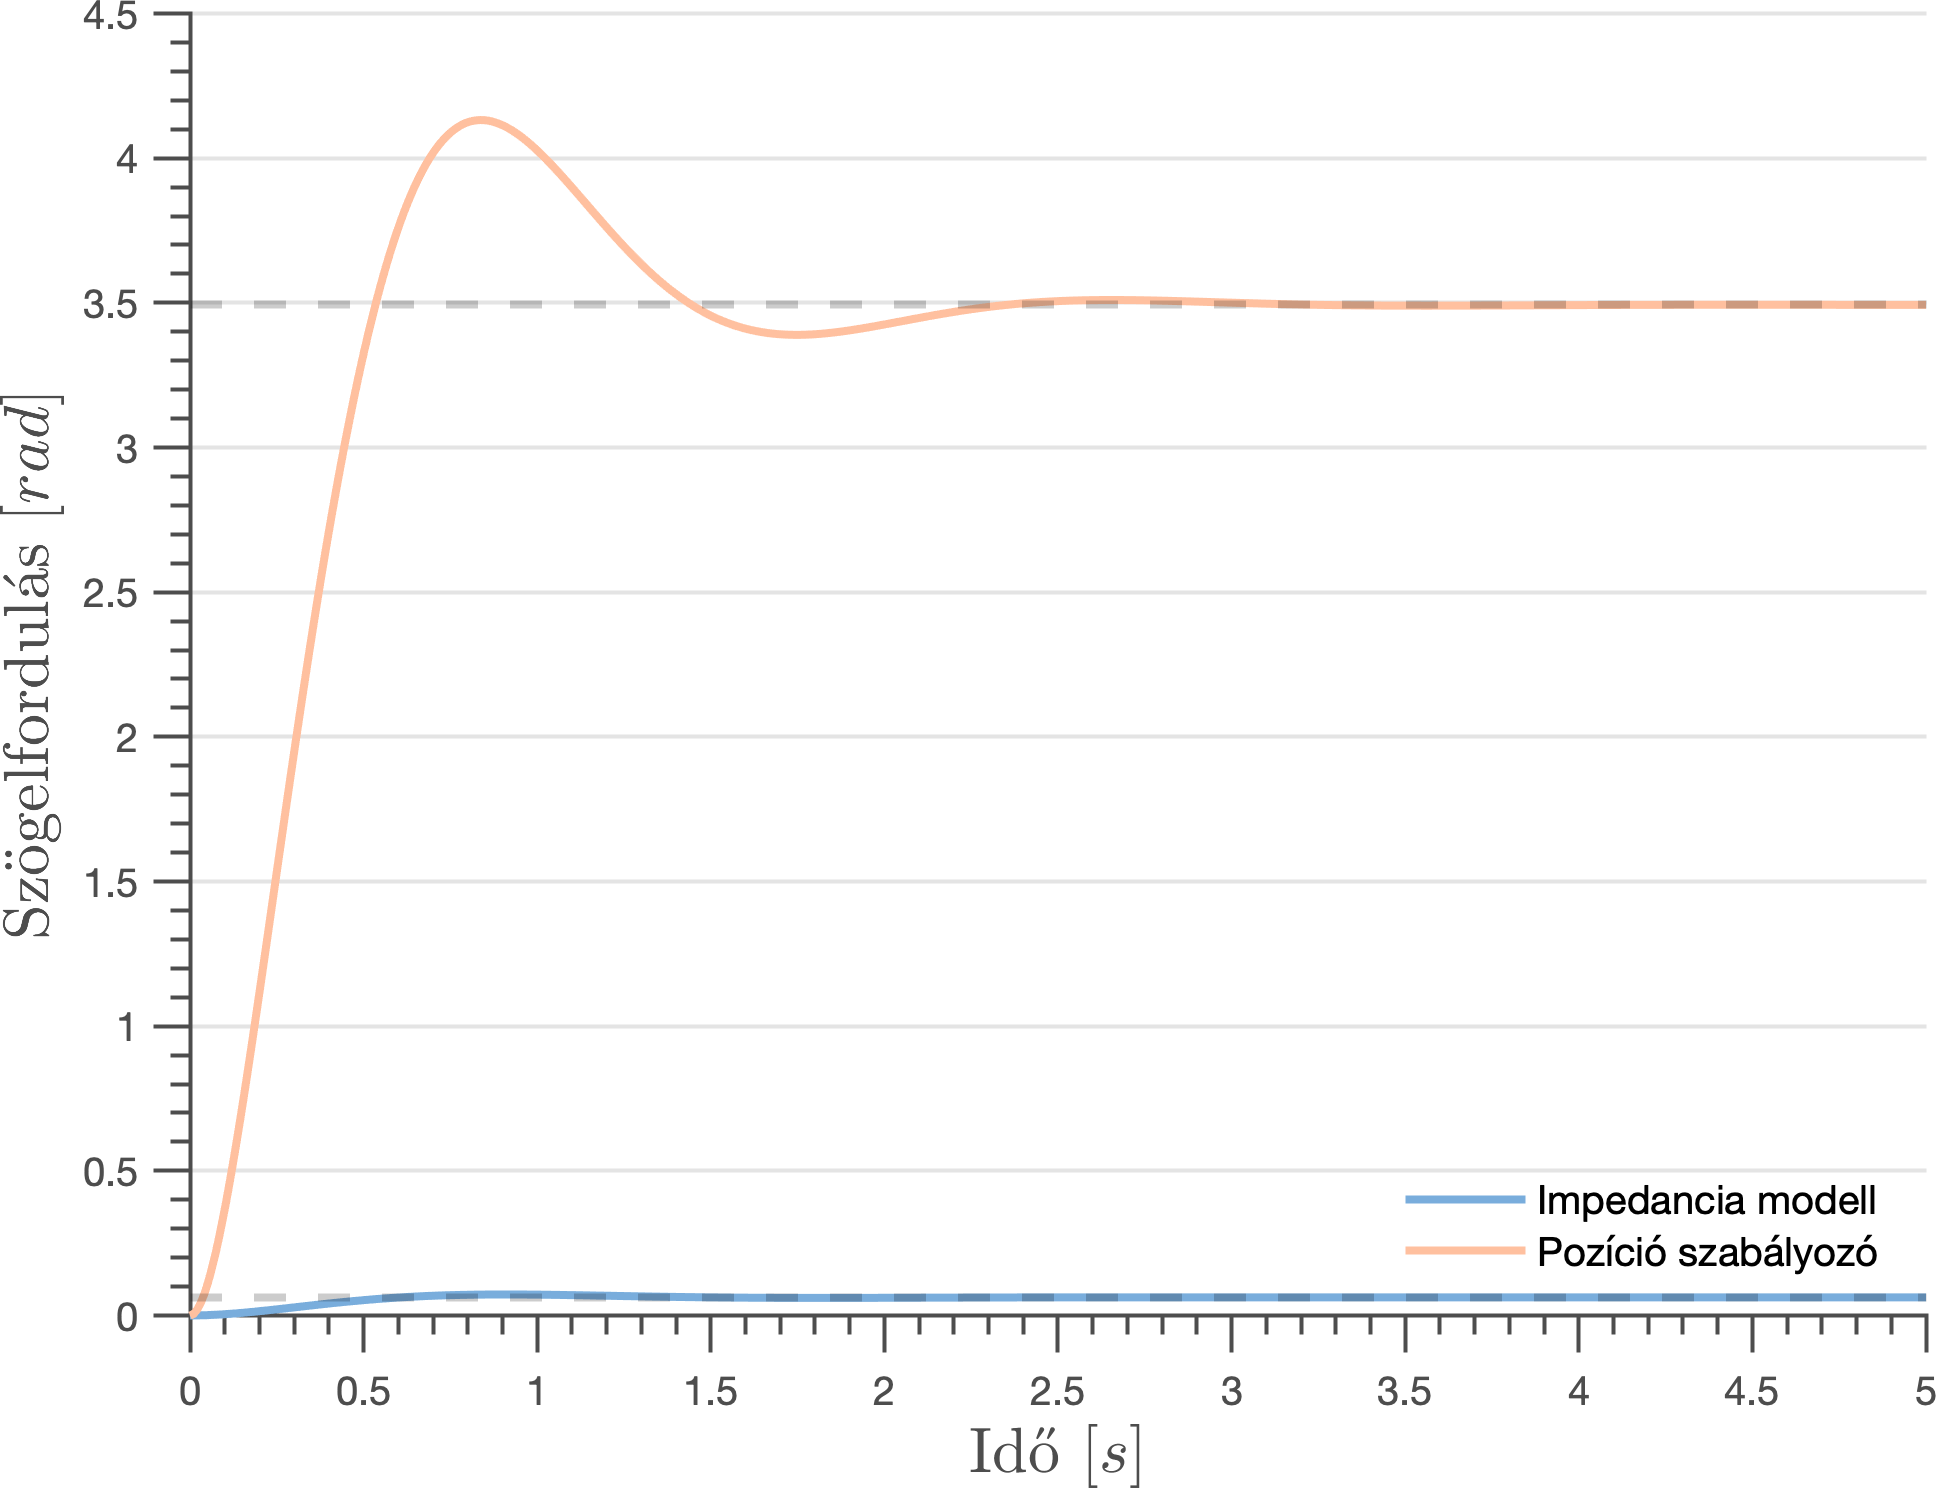
\includegraphics[width=\textwidth]{images/observer_controller_torque_resp.png}
    \caption{Az impedancia modell és a szabályozó összehasonlítása külső nyomaték egységugrás bemenetre}\label{fig:observer_controller_torque_resp}
    \end{center}
\end{figure}

\section{Nyomaték kompenzáció}
A rendszer válasza a külső nyomaték bemenetre adott egységugrás jelre a~\ref{fig:observer_controller_torque_resp}. ábrán látható. 
Az alkalmazott paraméterek a~\ref{tab:observer_controller_pos_resp}. táblazatban szerepelnek.
A végérték nem egyezik meg az impedancia modell által előírt értékkel, így további módosításokra van szükség.
A modell két bemenete közül csak a feszültségre van hatással a 
szabályozó, így a környezet által kifejtett külső nyomaték 
hatását is a feszültség megváltoztatásával kell kompenzálni. A kompenzáció
a külső nyomaték direkt vagy indirekt visszacsatolásával érhető el.
Direkt mérés esetén a külső nyomaték értékét egy szenzor adja meg.
A további vizsgálatok során feltételezett, hogy a szenzor dinamikája elhanyagolhatónak tekinthető. Az
állapotmegfigyelővel és kompenzációval ellátott rendszer teljes 
blokkdiagramját a~\ref{fig:block_diagram_direct_compensation}. ábra mutatja.
\begin{figure}[ht]
    \begin{center}
    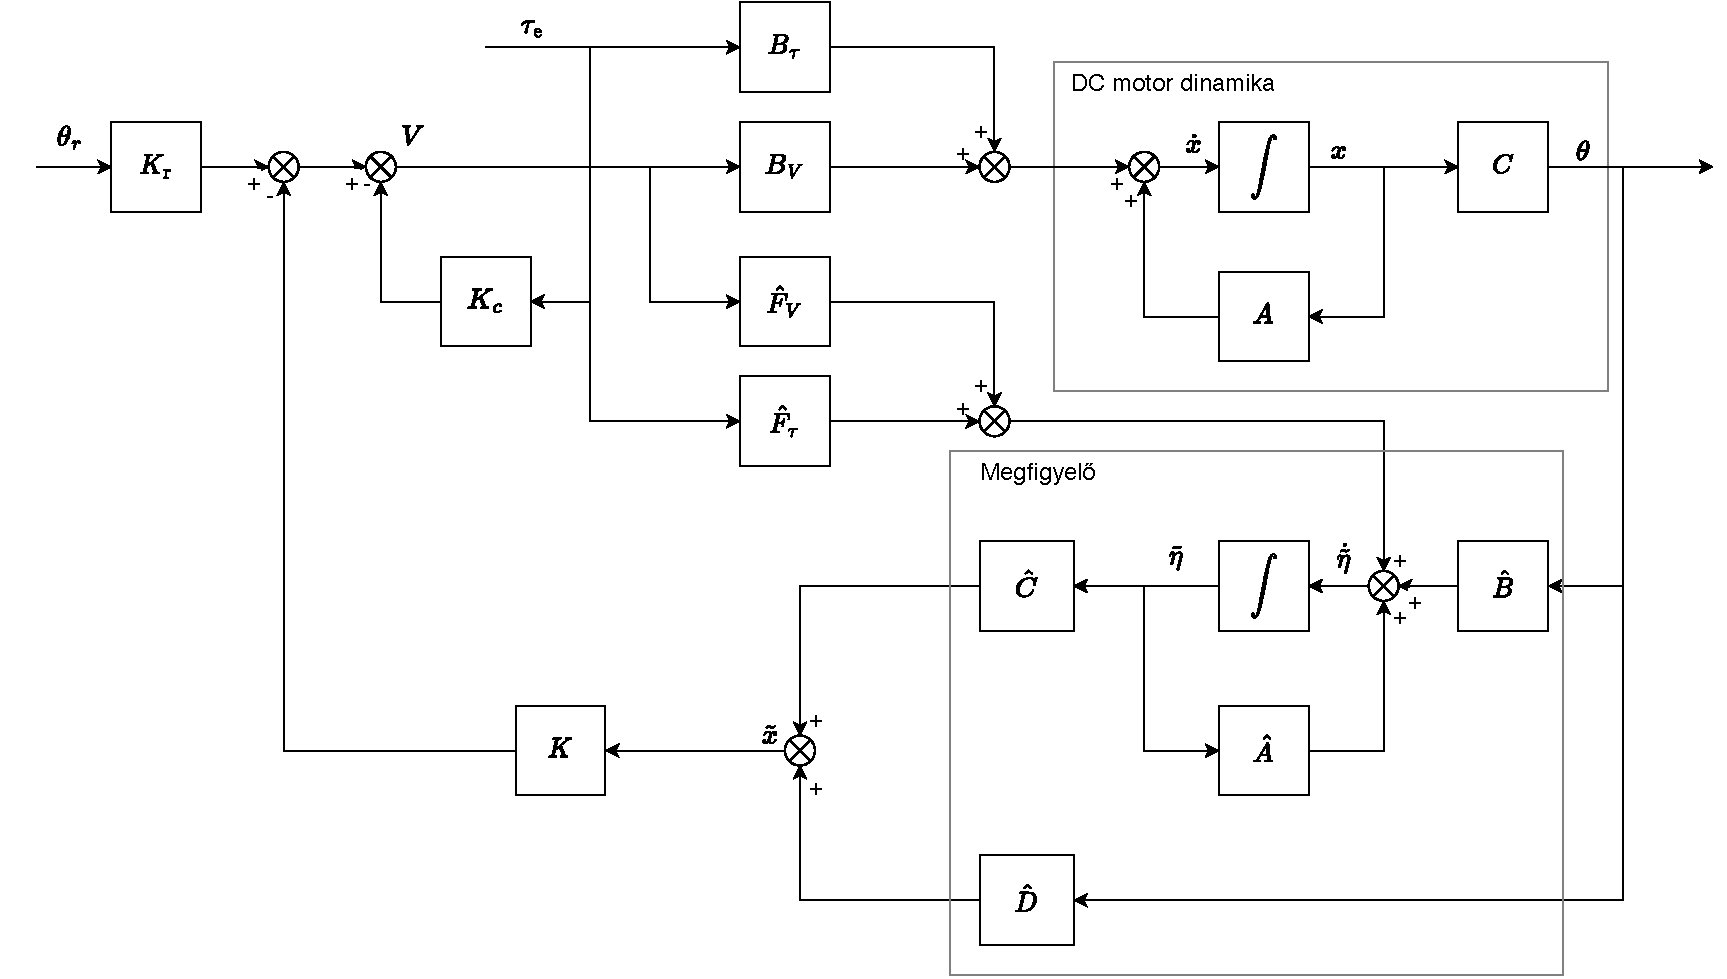
\includegraphics[width=\textwidth]{images/compensated_position_control_torque.pdf}
    \caption{Impedancia szabályozó közvetlen nyomaték méréssel}\label{fig:block_diagram_direct_compensation}
    \end{center}
\end{figure}

A kompenzált rendszernél alkalmazott visszacsatolási összefüggés az~\eqref{eq:position_control_voltage}. egyenlethez
hasonló, azonban megjelenik a mért külső nyomaték:
\begin{align}
    V = K_\RM r \theta_\RM r - K_\RM c \tau_\RM e - \BF K \tilde{\BF x}\,,
\end{align}
ahol $\BF K$ az állapot visszacsatolási mátrix, $K_\RM c$ a nyomaték kompenzációs együttható,
$K_\RM r$ a bemeneti erősítési tényezője és $\theta_\RM r$ az előírt szögelfordulás.
A pozíció szabályozónál alkalmazott levezetéshez hasonlóan meghatározható a módosított rendszer teljes dinamikája.
A visszacsatolási összefüggést behelyettesítve az~\eqref{eq:state_space_generic}. egyenletbe:
\begin{align}\label{eq:state_control_law_subs}
    \dot{\BF x} = \BF A \BF x + \BF B_\RM V\left[-\BF K \tilde{\BF x} -K_\RM c \tau + K_\RM r \theta_\RM r\right] + \BF B_\RM \tau \tau\,,
\end{align}
mely a becsült és a valódi állapotok közötti hibával kifejezve 
\begin{align}
    \dot{\BF x} = \left(\BF A - \BF B_\RM V \BF K\right) \BF x + 
    \BF B_\RM V \BF K \BF e + 
    \left(\BF B_\RM \tau - \BF B_\RM V K_\RM c\right) \tau + 
    \BF B_\RM V K_\RM r \theta_\RM r\,,
\end{align}
alakra hozható. A megfigyelő bemenetét kiegészítve a mért külső nyomatékkal:
\begin{equation}
    \begin{split}
    \dot{\BF x}_\RM b &= \BF A_\RM{ba} x_\RM a + \BF A_\RM{bb} \BF x_\RM b + 
    \BF B_\RM{Vb} V + \BF B_\RM{\tau b} \tau_\RM e\,,\\
    \dot{\tilde{\BF x}}_\RM b &= \left(\BF A_\RM{bb} - \BF K_\RM e \BF A_\RM{ab}\right) \tilde{\BF x}_\RM b +
    \BF A_\RM{ba} x_\RM a +
    \BF K_\RM e \BF A_\RM{ab} \BF x_\RM b +
    \BF B_\RM{Vb} V + \BF B_\RM{\tau b} \tau_\RM e\,,
    \end{split}
\end{equation}
melyeket kivonva egymásból
\begin{align}
    \dot{\BF e} = \left(\BF A_\RM{bb} - \BF K_\RM e \BF A_\RM{ab}\right) \BF e\,.
\end{align}
A rendszer dinamikája blokk mátrix alakban
\begin{align}
    \begin{bmatrix}
        \dot{\BF x} \\
        \dot{\BF e}
    \end{bmatrix}
    =
    \begin{bmatrix}
        \BF A - \BF B_\RM V \BF K & \BF B_\RM V \BF K_\RM b \\
        \BF 0 & \BF A_\RM{bb} - \BF K_\RM e \BF A_\RM{ab}
    \end{bmatrix}
    \begin{bmatrix}
        \BF x \\
        \BF e
    \end{bmatrix}
    +
    \begin{bmatrix}
        \BF B_\RM \tau - \BF B_\RM V K_\RM c & \BF B_\RM V K_\RM r\\
        \BF 0 & \BF 0
    \end{bmatrix}
    \begin{bmatrix}
        \tau_\RM e \\
        \theta_\RM r
    \end{bmatrix}.
\end{align}

A megfigyelő belső hibájának megváltozása csak a pillanatnyi belső hibától függ. A rendszer 
kimenete alapján megfigyelhető a belső állapota, a \(\BF K_\RM e\) mátrixot megfelelően kiválasztva
a rendszer belső hibáját tekintve exponenciálisan stabil. Hasonlóan mivel a rendszer teljesen irányítható,
a \(\BF K\) visszacsatolási mátrixot megfelelően kiválasztva a teljes rendszer is exponenciálisan stabil.

Indirekt nyomaték visszacsatolás kontextusában (a rendszer szöggyorsulásának mérése alapján) 
a~\ref{fig:block_diagram_indirect_compensation}. ábra mutatja a teljes blokkdiagramot.
\begin{figure}[ht]
    \begin{center}
    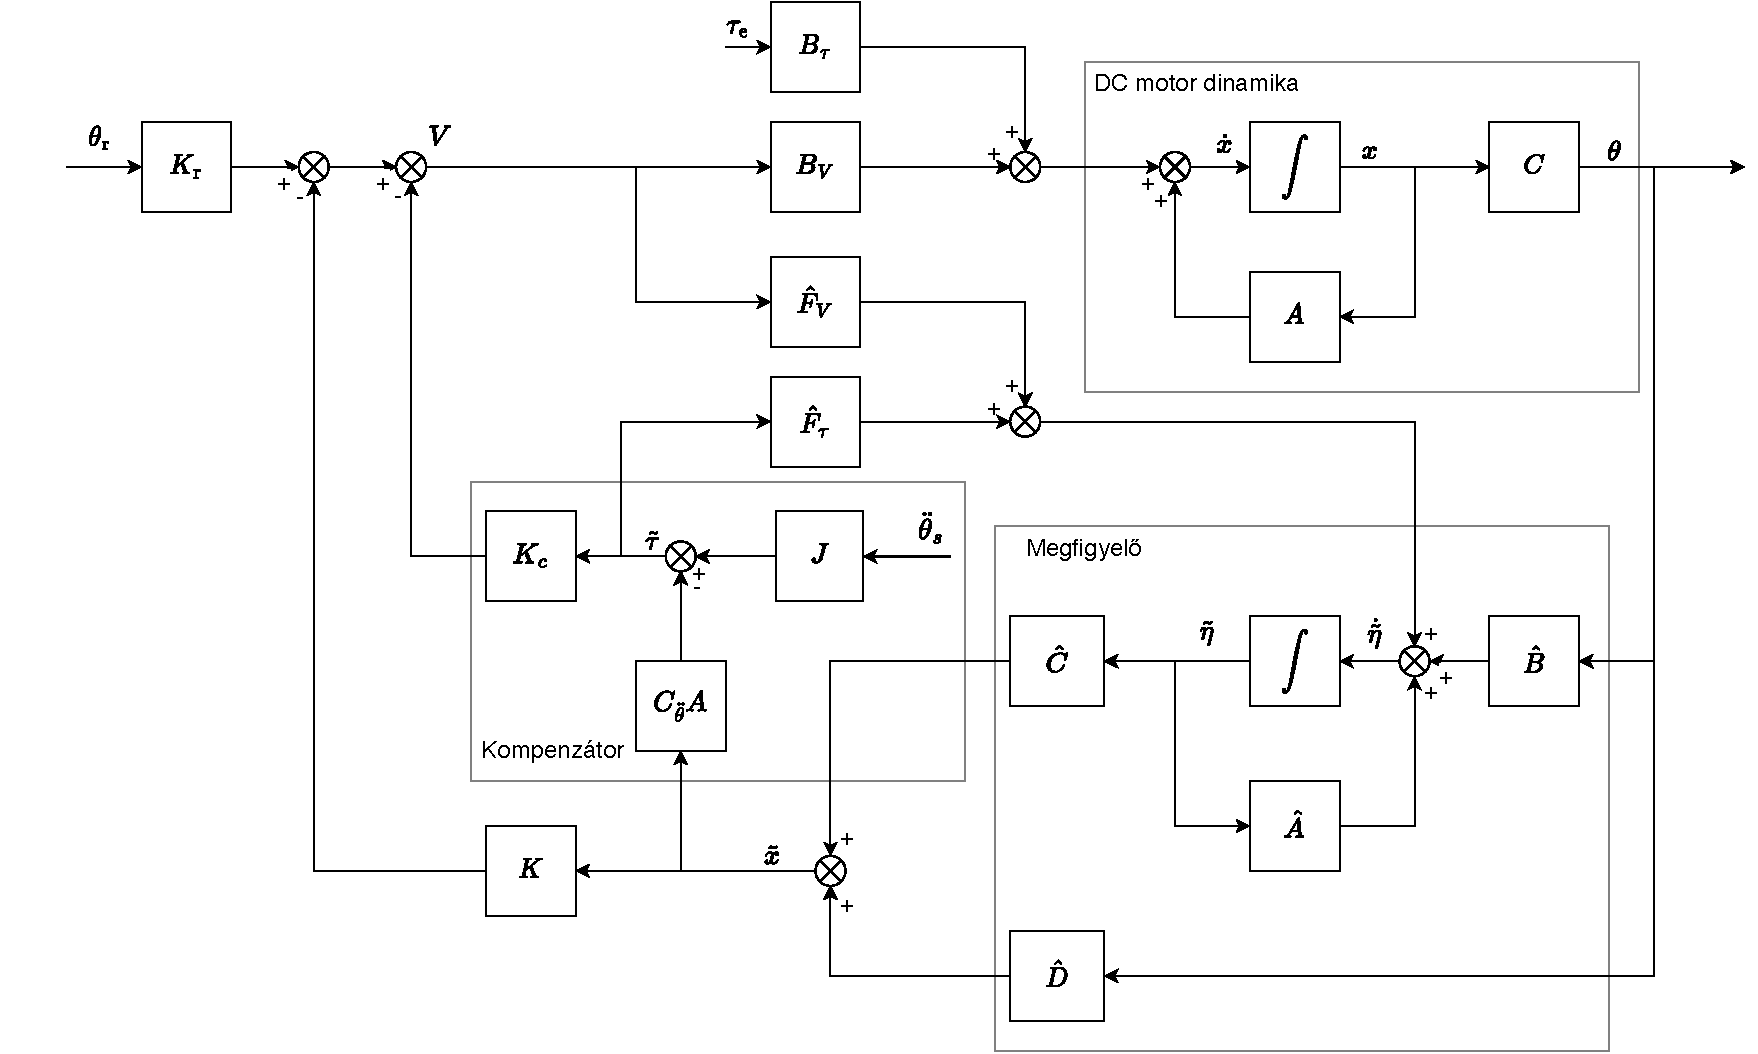
\includegraphics[width=\textwidth]{images/compensated_position_controller_angular_acceleration.pdf}
    \caption{Impedancia szabályozó szöggyorsulás méréssel}\label{fig:block_diagram_indirect_compensation}
    \end{center}
\end{figure}
Ekkor egy becsült nyomaték érték kerül visszacsatolásra:
\begin{align}
    \tilde \tau = J \ddot \theta_\RM s - \BF C_{\ddot\theta} \BF A \tilde{\BF x}\,,
\end{align}
ahol \(\ddot \theta_\RM s\) a forgorész mért szöggyursulása és \(\BF C_{\ddot\theta} = [0~~1~~0]\).
alakban, a becsült állapot és a mért szöggyorsulás kombinációjával adható meg.
A feszültségjel a becsült nyomatékértékkel:
\begin{align}
    V = K_\RM r \theta_r - K_c \tilde \tau - \BF K \tilde{\BF x}.
\end{align}
Az előző levezetéshez hasonlóan meghatározható a teljes rendszer dinamikája:
\begin{align}
    \begin{bmatrix}
        \dot{\BF x} \\
        \dot{\BF e}
    \end{bmatrix}
    =
    \begin{bmatrix}
        \BF A - \BF B_\RM V \BF K & \BF B_\RM V (\BF K_\RM b - \BF C_{\ddot\theta} \BF A_\RM{*b} K_\RM c) \\
        \BF 0 & \BF A_\RM{bb} - \BF B_\RM{\tau b} \BF C_{\ddot\theta} \BF A_\RM{*b} - \BF K_\RM e \BF A_\RM{ab}
    \end{bmatrix}
    \begin{bmatrix}
        \BF x \\
        \BF e
    \end{bmatrix}
    +
    \begin{bmatrix}
        \BF B_\RM \tau - \BF B_\RM V K_\RM c & \BF B_\RM V K_\RM r\\
        \BF 0 & \BF 0
    \end{bmatrix}
    \begin{bmatrix}
        \tau_\RM e \\
        \theta_\RM r
    \end{bmatrix}.
\end{align}

A megfigyelő visszacsatolási mátrixának kiválasztása valamelyest módosul, de a megfelelő mátrixokkal
a rendszer továbbra is exponenciálisan stabil. Ebben az alkalmazásban direkt mérés alapján kerül meghatározásra
a rendszerre ható külső nyomaték, így a továbbiakban a~\ref{fig:block_diagram_direct_compensation}. ábrán
látható modell vizsgálata fog folytatódni.

A kompenzáció csak akkor lehet eredményes, ha a modellezett motor feszültség és külső nyomaték hatására is 
egyaránt közel azonos sebességgel reagál. A direkt nyomaték méréssel kompenzált modell válasza egységugrás
bemenetre a~\ref{fig:observer_controller_pos_resp_direct}. és~\ref{fig:observer_controller_torque_resp_direct}. ábrán látható. 
A felhasznált paraméterek továbbra is azonosak a kompenzálás nélküli modellnél alkalmazott paraméterekkel.
A nyomaték kompenzációs együttható
\begin{equation}
    K_\RM c = L\frac{- B_\RM m M_\RM e + B_\RM e J - J M_\RM e p + J^2 p}{J K_\RM m M_\RM e}
\end{equation}
összefüggés szerint számolható.
A pozíció referencia jelre adott válasz változatlan, azonban a külső nyomatékra adott válasz végértéke már
megegyezik az impedancia modell által előírt értékkel. A válaszban megfigyelhető túllövés kiküszöböléshez
a motor és az impedancia modell paraméterei, valamint a rendszer válasza közötti kapcsolat további vizsgálata szükséges.

\begin{figure}[ht]
    \begin{center}
    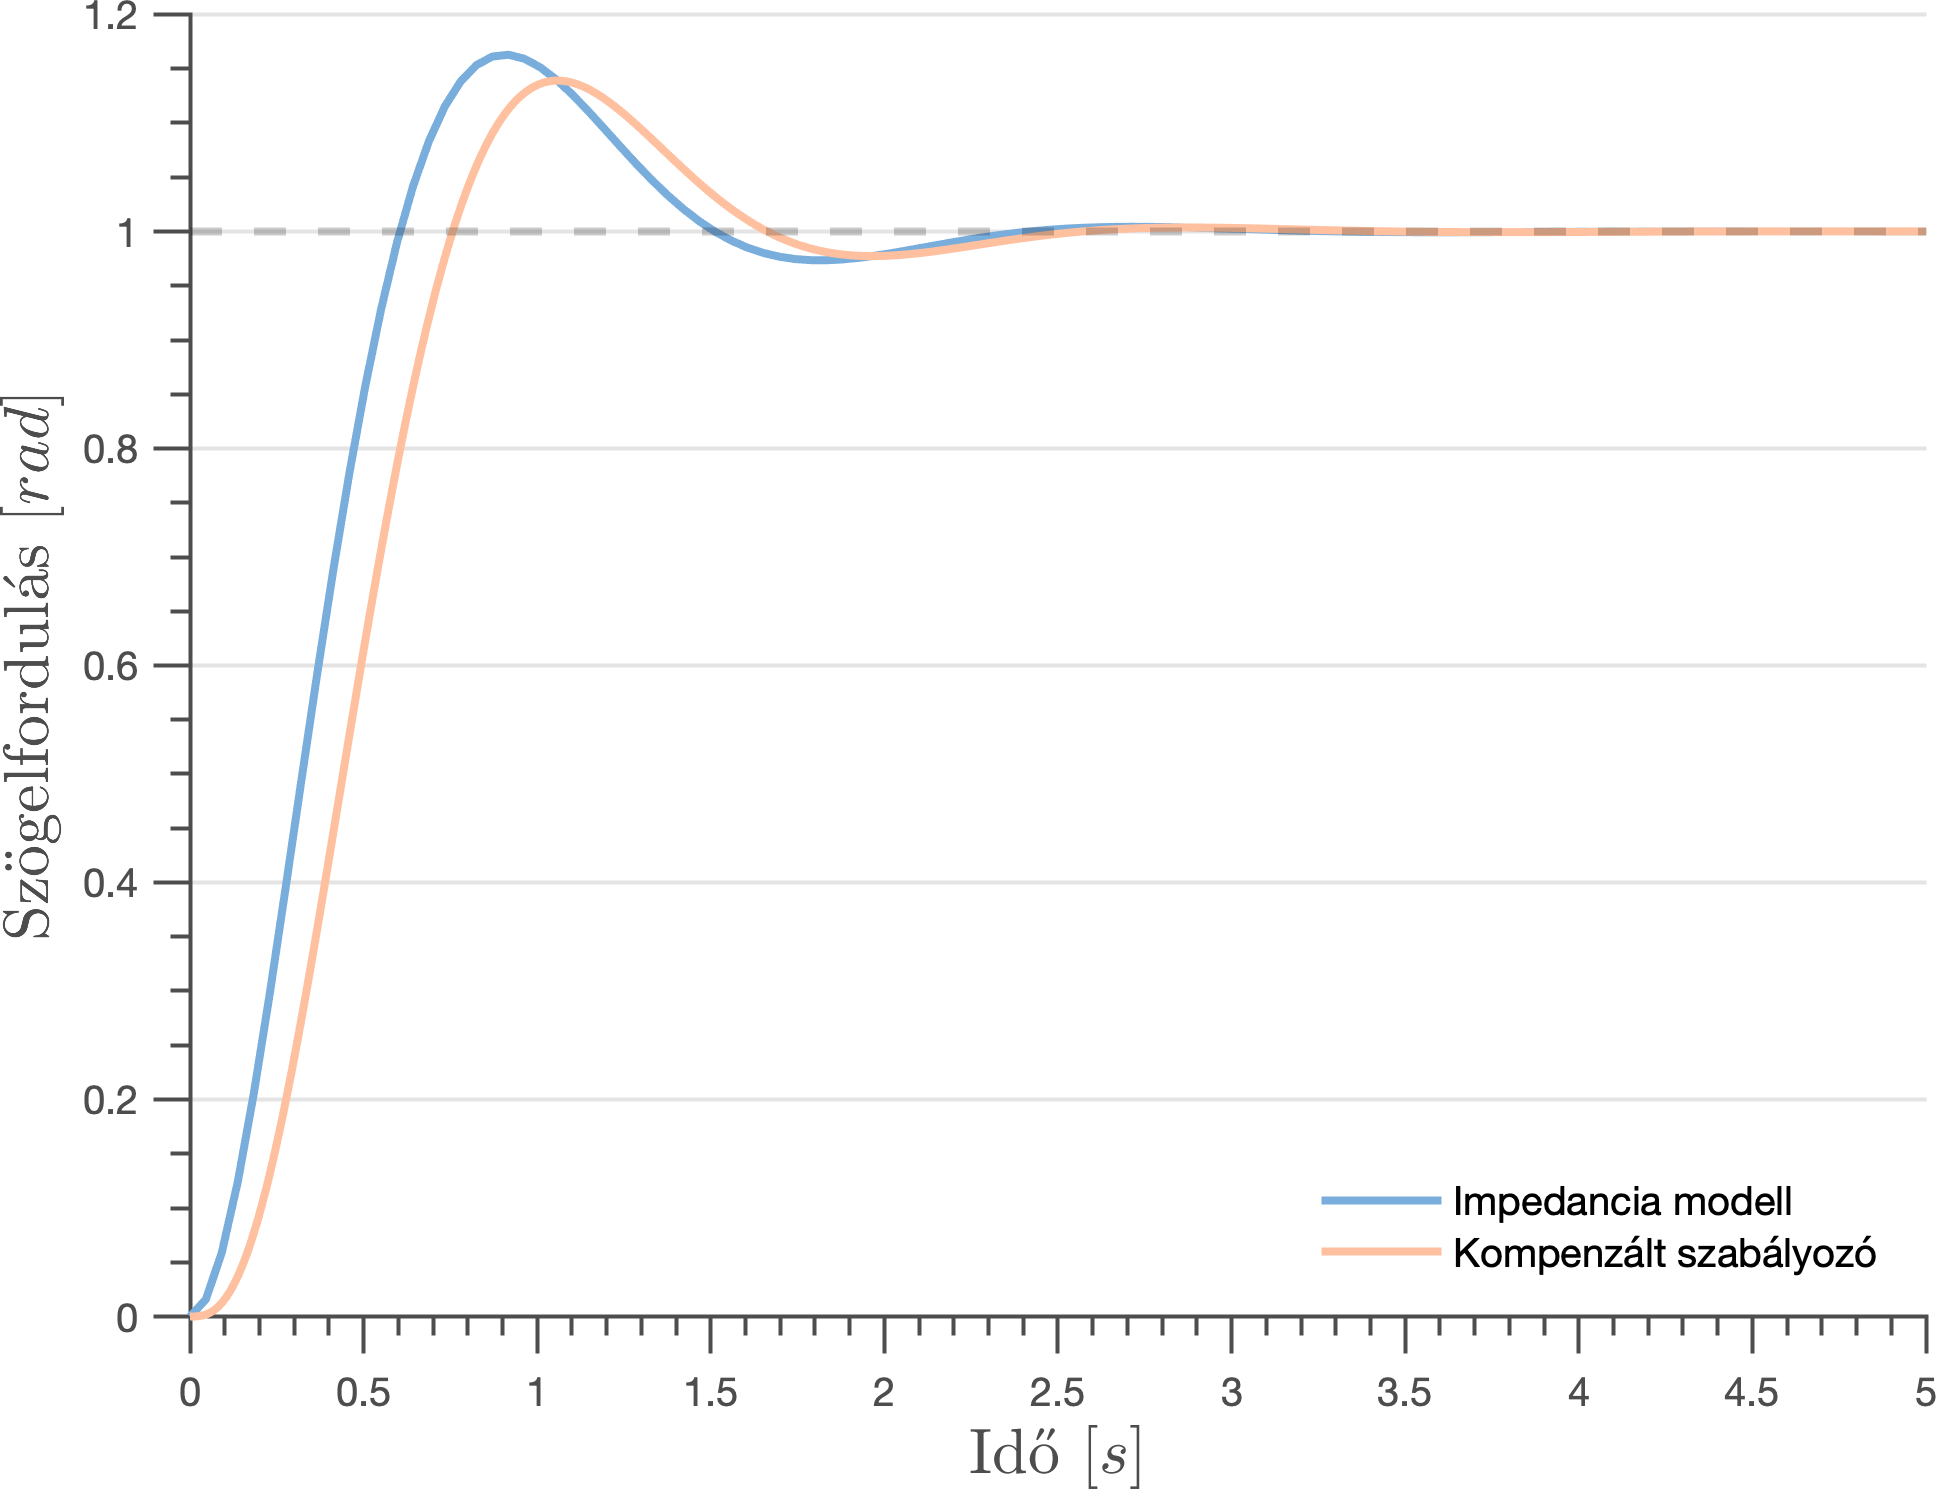
\includegraphics[width=\textwidth]{images/observer_controller_pos_resp_direct_comp.png}
    \caption{Az impedancia modell és a kompenzált szabályozó összehasonlítása pozíció egységugrás bemenetre}\label{fig:observer_controller_pos_resp_direct}
    \end{center}
\end{figure}

\begin{figure}[ht]
    \begin{center}
    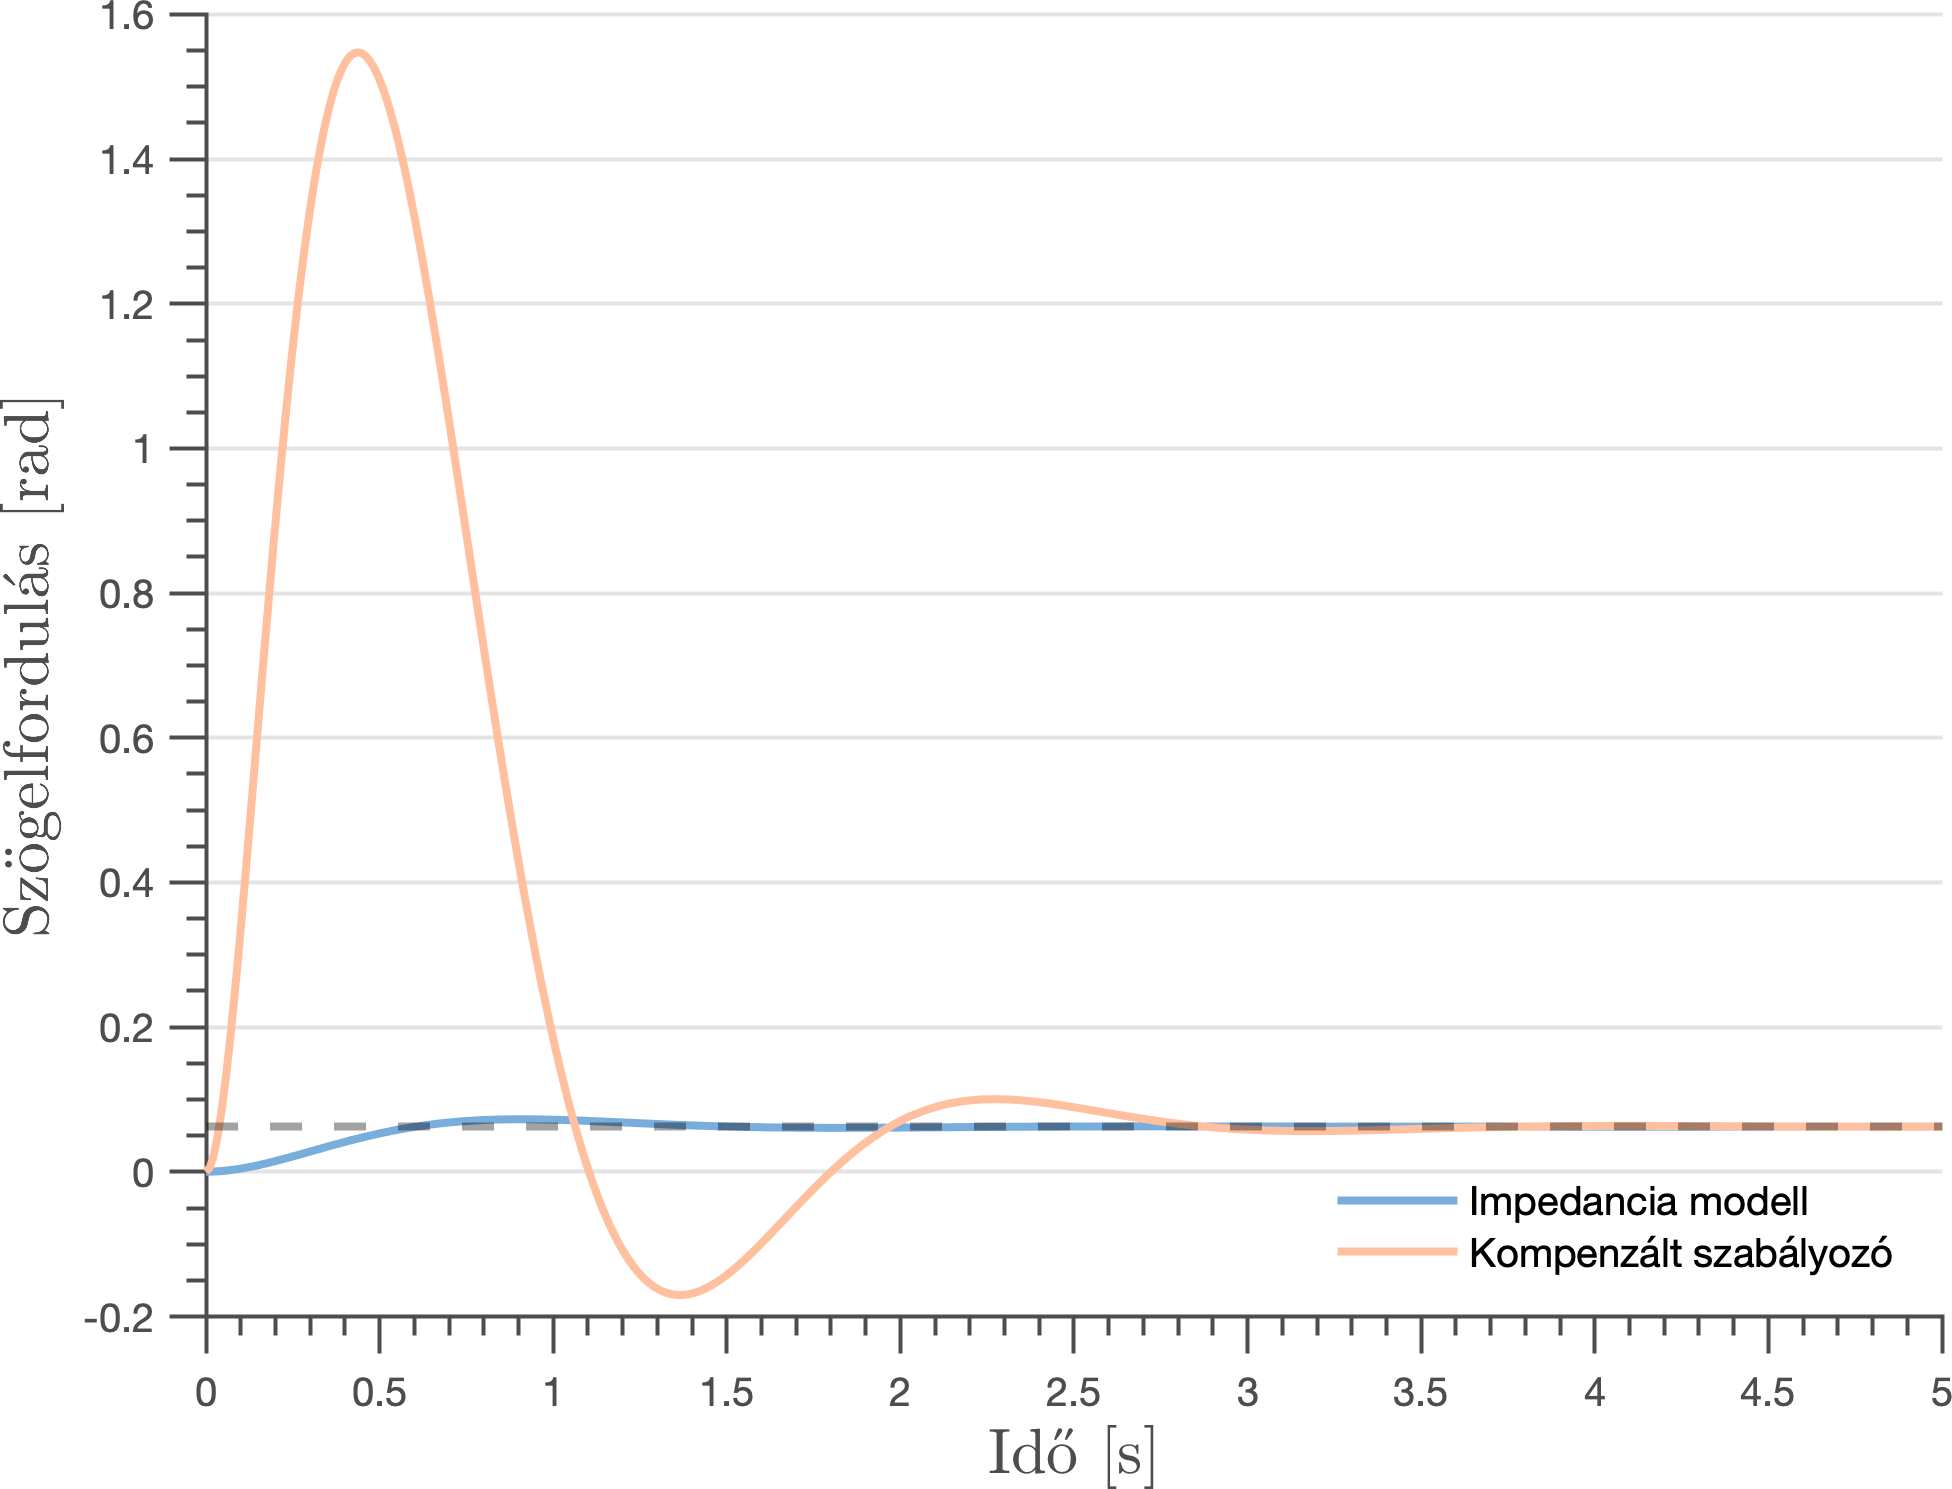
\includegraphics[width=\textwidth]{images/observer_controller_torque_resp_direct_comp.png}
    \caption{Az impedancia modell és a kompenzált szabályozó összehasonlítása külső nyomaték egységugrás bemenetre}\label{fig:observer_controller_torque_resp_direct}
    \end{center}
\end{figure}

Először is az impedancia modell paraméterei mind valós pozitív értékkel kell rendelkezzenek, enélkül a rendszer 
azonnal instabil lesz. Ez a Routh--Hurwitz kritérium alapján következik az impedancia modell karakterisztikus egyenletéből.
Az áthelyezett pólusok közül az első kettőt az impedancia modell előírt értékei határozzák meg. 
A harmadik áthelyezett pólus, illetve a megfigyelő pólusai függetlenek. A független pólusok meghatározásához 
mindegyik azonos lesz és valós értékű. Ha a pólusok túl közel helyezkednek el az impedancia modell pólusaihoz,
esetleg még a képzetes tengelyhez is közelebb vannak, akkor eltorzítják a választ. Ha túl nagy negatív valós
értékkel rendelkeznek, az a szabályozó kimenetének szaturációjához vezet, illetve magát a szabályozót is
instabillá teszik. Ennek elkerülése érdekében a lehető legkisebb abszolút értékű negatív valós pólus használata a cél. 
A rendszer átviteli függvénye a pozíció referencia jelet tekintve~\eqref{eq:input_coeff} felhasználásával:
\begin{align}
    \frac{\theta(s)}{\theta_\RM r (s)} = \frac{K_\RM e p}{(p-s)(M_\RM e s^2 + B_\RM e s + K_\RM e)}\,,
\end{align}
ahol \(p\) a keresett pólus. A pólus hatása közelíthető egy időkéséses taggal, mivel
\begin{align}
    e^{-\tau s} = 1 - \tau s + \cdots\,,
\end{align}
ahol \(\tau\) az időkésés, az átviteli függvény a következő késleltetett másodrendű rendszerrel közelíthető:
\begin{align}
    \frac{\theta(s)}{\theta_\RM r (s)} \approx \frac{K_\RM e}{M_\RM e s^2 + B_\RM e s + K_\RM e}e^{\frac{1}{p}s}\,,
\end{align}
tehát \(\tau = -\frac{1}{p}\) felhasználható a pólus maximumának meghatározásához. A továbbiakban 
ez az időkésés a rendszer beállási idejének legfeljebb 5\%-ára lesz korlátozva. Eszerint a pólus legfeljebb:
\begin{align}\label{eq:pole_selection_pos}
    p_\RM{max} = -\frac{1}{\frac{4}{\zeta \omega_0} \cdot 0.05} = -\frac{B_\RM e}{8M_\RM e \cdot 0.05}
\end{align}
lesz. A külső nyomatékra adott válasz időtartománybeli vizsgálata további feltételekhez vezet. 
Nem minden paraméterkombináció ad elfogadható választ, ahogy a~\ref{fig:observer_controller_torque_resp_direct}.
ábrán is látszik. A rendszer átviteli függvénye a külső nyomaték jelet tekintve:
\begin{align}
    \frac{\theta(s)}{\tau_\RM e (s)} = 
    \frac{Jp - M_\RM e s}{J(p-s)(M_\RM e s^2 + B_\RM e s + K_\RM e)} = 
    \frac{1 -\frac{M_\RM e}{Jp} s}{(1-\frac{1}{p}s)(M_\RM e s^2 + B_\RM e s + K_\RM e)}\,,
\end{align}
hasonlóan az előző feltételhez a függvény közelíthető egy késleltetett másodrendű rendszerrel. A válaszban 
megjelenik a bemenet deriváltja. Hatásának korlátozása ad újabb maximumot a független pólusok értékére. A 
továbbiakban a bemeneti jel deriváltjának együtthatója legalább egy nagyságrenddel kisebb kell legyen egynél.
Ebből következik, hogy a pólus értékének maximuma:
\begin{align}\label{eq:pole_selection_torque}
    p_\RM{max} = -10 \cdot \frac{M_\RM e}{J}
\end{align}
A két feltétel együtt azt eredményezi, hogy a pólus értéke abszolút értékben a lehető legkisebb, amikor
az előírt tehetetlenség és a pólus értékének maximuma:
\begin{equation}\label{eq:pole_selection_extremum}
    \begin{split}
        M'_\RM e &= 0.5 \cdot \sqrt{JB_\RM e}\,, \\
        p'_\RM{max} &= -5 \cdot \sqrt{\frac{B_\RM e}{J}}\,.
    \end{split}
\end{equation}
A szaturáció elkerüléséhez szükséges feltételek részletes vizsgálata túlmutat ezen a dolgozaton, azonban feltételezhetően 
a pólusválasztásnál van egy minimum érték mely alatt a rendszer nem képes követni az impedancia modellt. Jelölje \(p_\RM{min}\) ezt a 
minimumot. Ekkor az előírt tehetetlenség lehetséges értékei a~\eqref{eq:pole_selection_pos}. és a~\eqref{eq:pole_selection_torque} 
egyenletekben szereplő feltételek szerint egy adott intervallumra korlátozódnak:
\begin{align}
    -\frac{B_\RM e}{8p_\RM{min} \cdot 0.05} < M_\RM e < -0.1 \cdot Jp_\RM{min}\,,
\end{align}
illetve az előírt viszkózus csillapítási együtthatóra is adódik egy maximális korlát~\eqref{eq:pole_selection_extremum} alapján:
\begin{align}
    B_\RM{e,max} = 0.04 \cdot Jp^2_\RM{min}\,,
\end{align}
ami felett nem választható ki olyan pólus, mely a követelményeknek megfelelő választ eredményez. 
Egy adott \(p_\RM{min}\) minimum pólus értékre és \(J\) motor tehetetlenségre ábrázolja 
a választható tehetetlenség - pólus párokat a~\ref{fig:observer_controller_param_limits}. ábra.
A kontúrok konstans \(B_\RM e\) előírt viszkózus csillapítási tényezőket jelölnek a~\eqref{eq:pole_selection_pos}.
egyenlet szerint.

\begin{figure}[ht]
    \begin{center}
    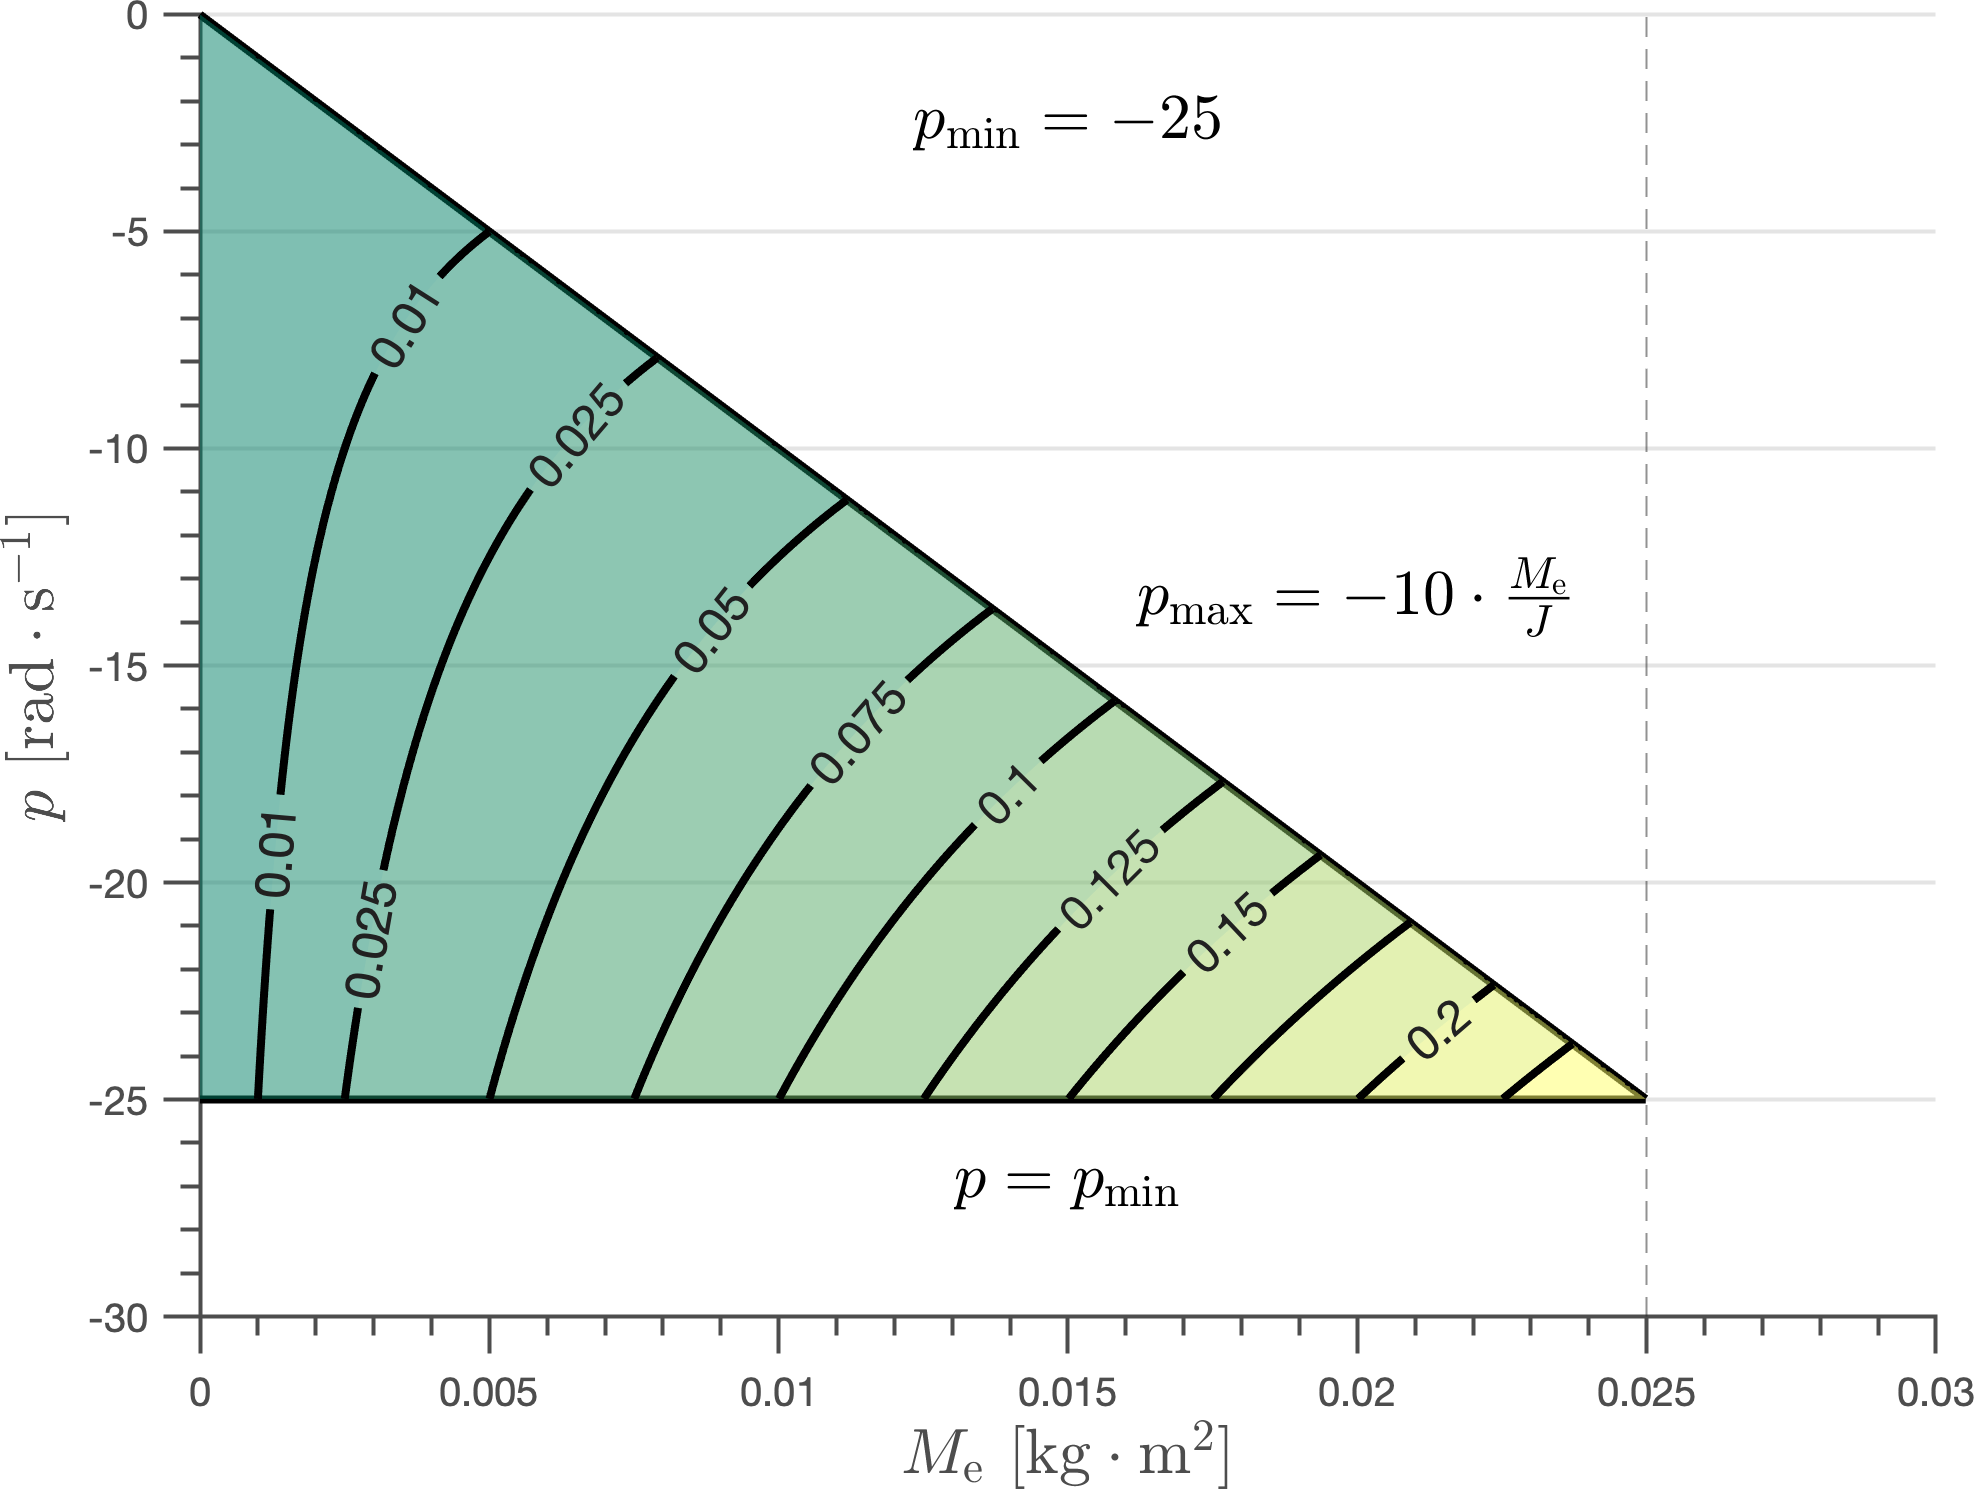
\includegraphics[width=\textwidth]{images/observer_controller_param_limits.png}
    \caption{Az előírható tehetetlenség és a független pólus közötti összefüggés}\label{fig:observer_controller_param_limits}
    \end{center}
\end{figure}

Az előző feltételek alapján a pozíció referencia jelre és  külső nyomaték hatására is megfelelő válasz kapható.
Egy ilyen válasz látható a~\ref{fig:observer_controller_pos_resp_direct_calib}. 
és a~\ref{fig:observer_controller_torque_resp_direct_calib} ábrán. 
Az alkalmazott paramétereket a~\ref{tab:observer_controller_pos_resp_calib}. táblazat tartalmazza.

\begin{table}[ht]
    \small\centering
    \caption{A kalibrált szabályozónál alkalmazott paraméterek}\label{tab:observer_controller_pos_resp_calib}
    \tabcolsep=1pt
    \begin{tabular}{l>{~}l>{\quad}rl}
        \toprule
        \multicolumn{2}{c}{Szimbólum és paraméter név} & \multicolumn{2}{c}{Érték} \\ \midrule
        \(M_\RM e\) & Előírt tehetetlenség & 0.015 & \(\RM{kg\cdot m^2}\) \\
        \(B_\RM e\) & Előírt viszkózus csillapítás & 0.06 & \(\RM{kg\cdot m^2\cdot s^{-1}}\) \\
        \(K_\RM e\) & Előírt rugóállandó & 0.24 & \(\RM{kg\cdot m^2\cdot s^{-2}}\) \\
        \(J\) & Motor tehetetlensége & 0.01 & \(\RM{kg\cdot m^2}\) \\
        \(K_\RM m\) & Motor nyomatékállandója & 0.01 & \(\RM{Nm\cdot A^{-1}}\) \\
        \(B_\RM m\) & Motor modell viszkózus csillapítása & 0.1 & \(\RM{kg\cdot m^2\cdot s^{-1}}\) \\
        \(L\) & Motor induktivitása & 0.2 & H \\
        \(R\) & Motor ellenállása & 1 & \(\Omega\) \\
        \(p\) & További pólusok & -15 & \(\RM{rad \cdot s^{-1}}\) \\
        \(K_\RM c\) & Nyomaték kompenzációs együttható & -50 & \(\RM{V \cdot N^{-1} m^{-1}}\) \\
        \bottomrule
    \end{tabular}
\end{table}
\begin{figure}[ht]
    \begin{center}
    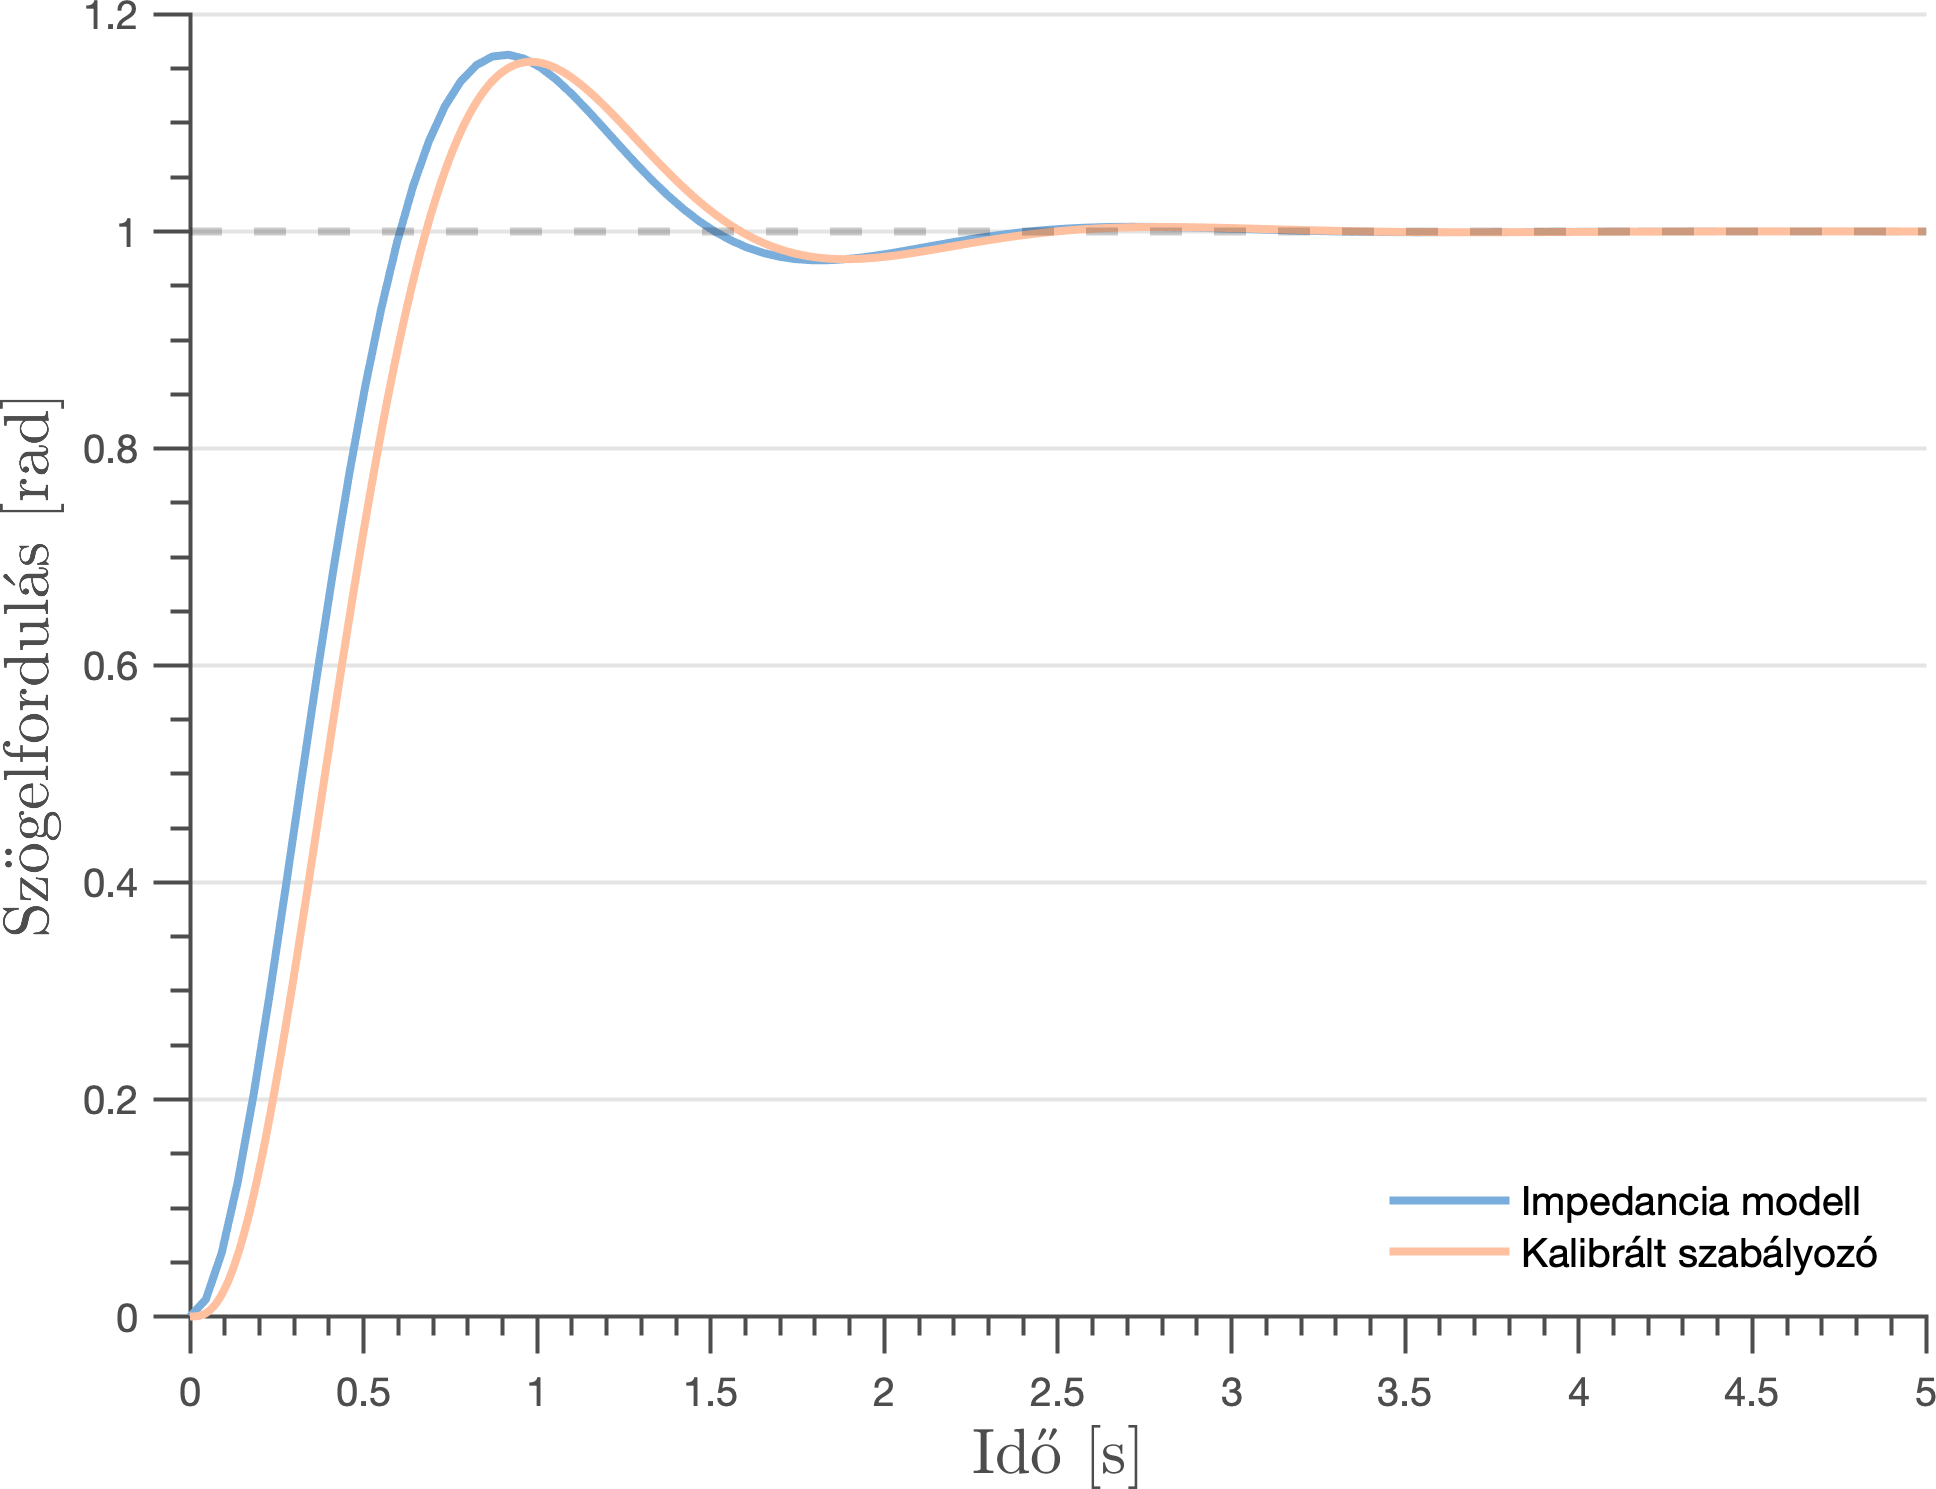
\includegraphics[width=13cm]{images/observer_controller_pos_resp_direct_comp_calib.png}
    \caption{Az impedancia modell és a kalibrált szabályozó összehasonlítása pozíció egységugrás bemenetre}\label{fig:observer_controller_pos_resp_direct_calib}
    \end{center}
\end{figure}

\begin{figure}[ht]
    \begin{center}
    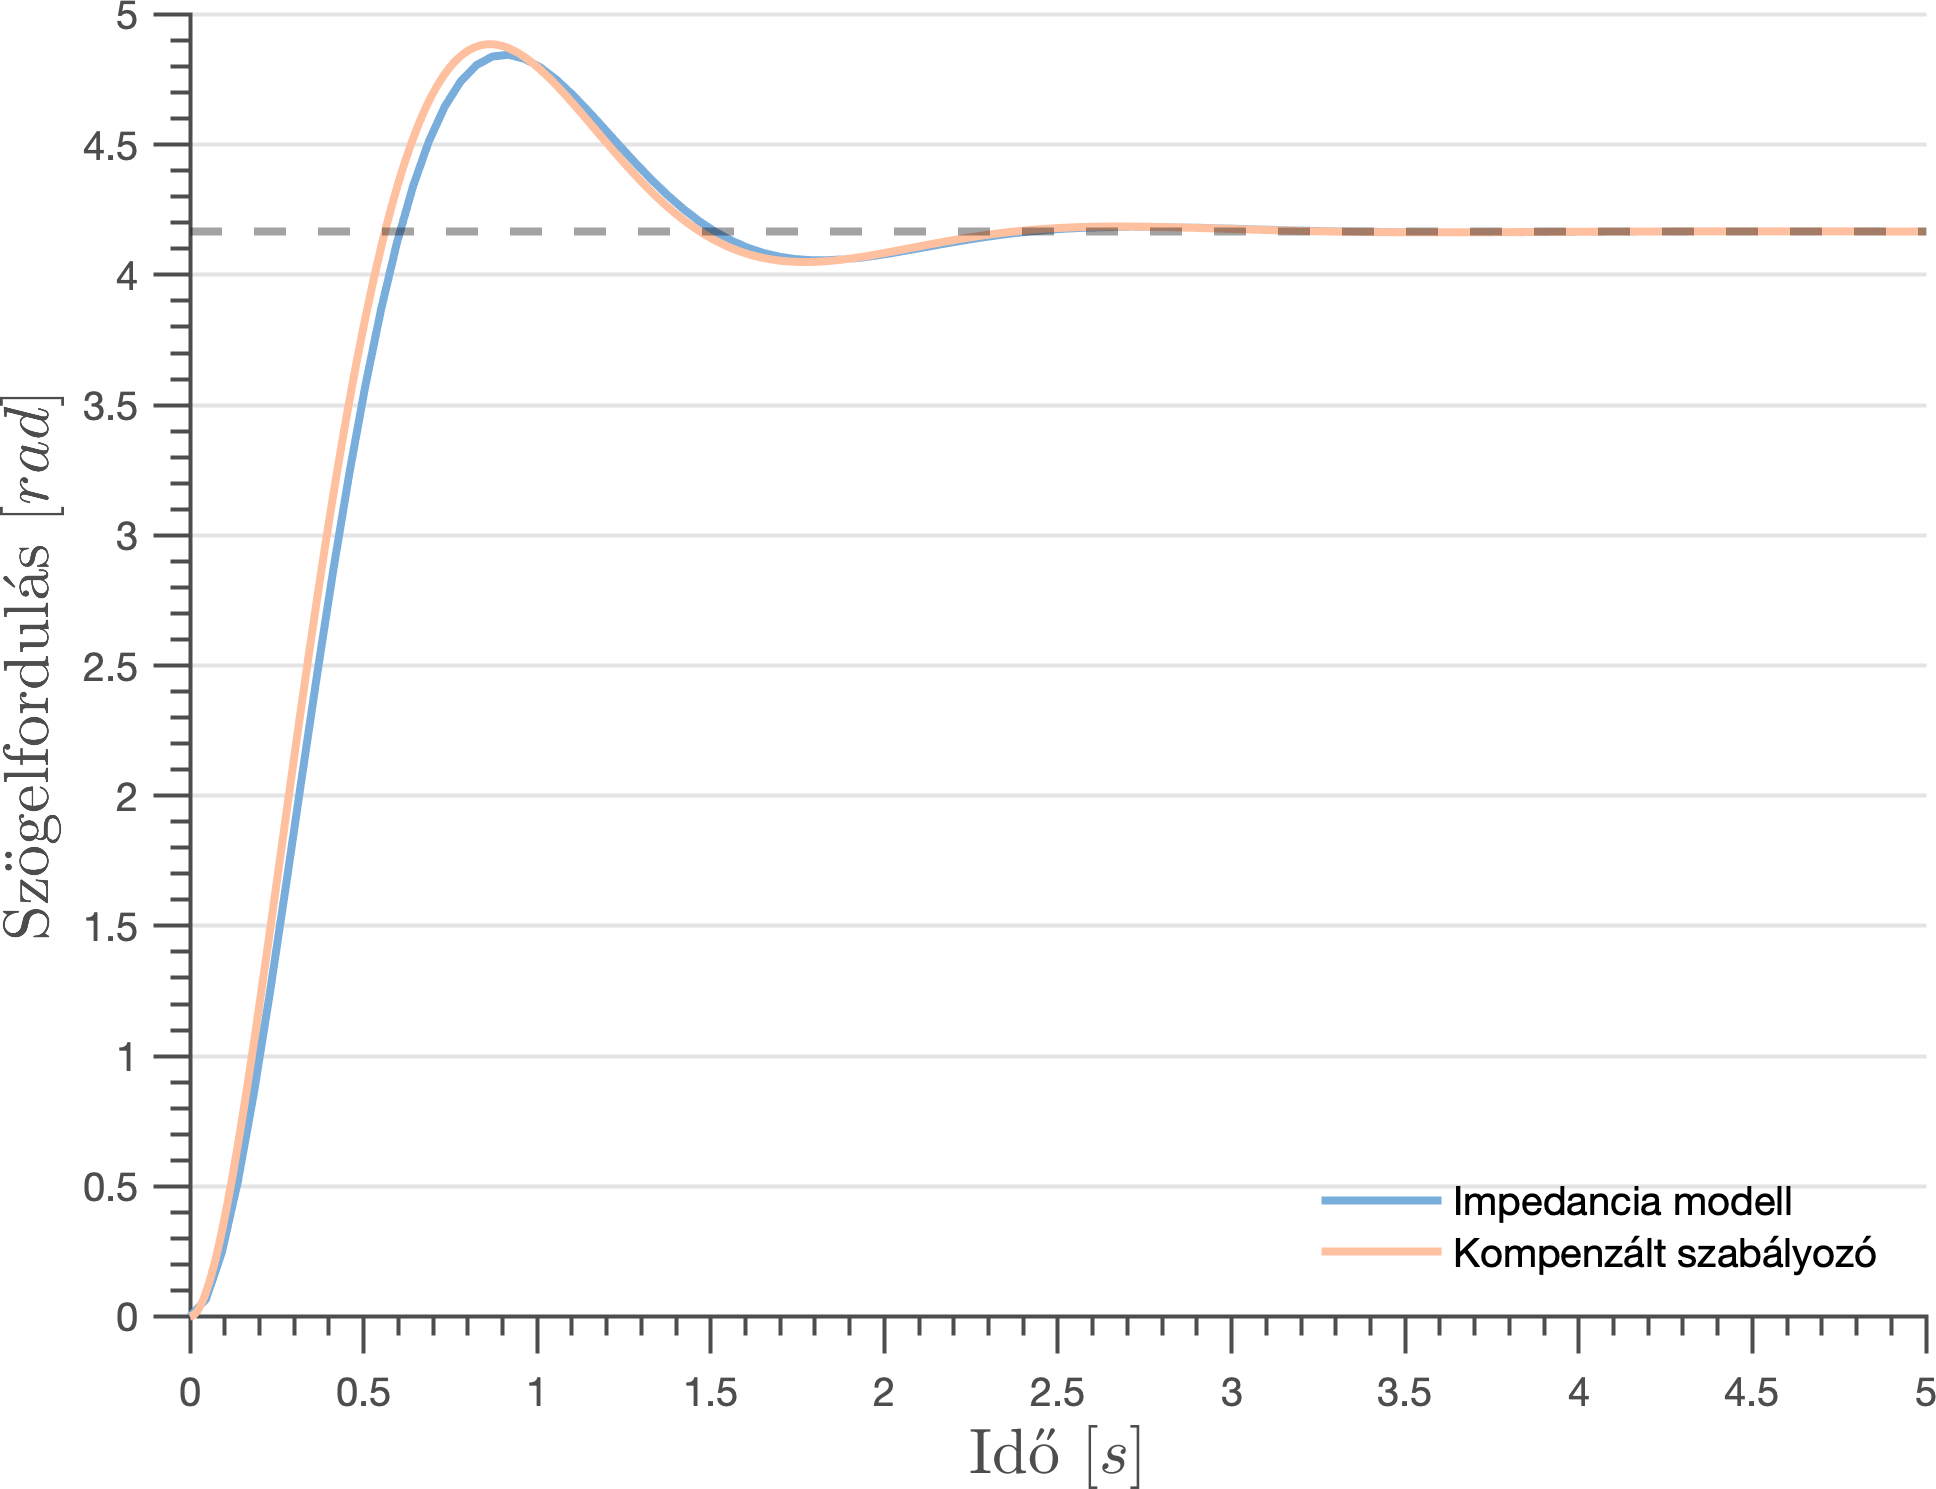
\includegraphics[width=13cm]{images/observer_controller_torque_resp_direct_comp_calib.png}
    \caption{Az impedancia modell és a kalibrált szabályozó összehasonlítása külső nyomaték egységugrás bemenetre}\label{fig:observer_controller_torque_resp_direct_calib}
    \end{center}
\end{figure}

Az impedancia modell előírt rugóállandójára az előző elemzés nem ad korlátot, viszont 
ennek a paraméternek a növelésével növekszik a modell sajátfrekvenciája. Ez mindenképp 
egyre nagyobb előrt gyorsulással jár, mely a motorra kapcsolt feszültség szaturációjához vezet.

Az áthelyezett pólusok értékeinek függvényében a szabályozó önmagában instabil lehet. Mivel a rendszer szabályozás 
nélkül instabil, mindenképp szükséges független biztonsági mechanizmus beépítése, így ennek az esetnek az elemzése elmarad. 
